\clearpage
\section{Softwarové zpracování}
\indent\indent Signály převedené do nízkofrekvenčního pásma jsou navzorkovány zvukovou kartou a následně v reálném čase zpracovávané programem.
\subsection{Základní princip zpracování}
\indent\indent Program nejprve převede přijímaný signál pomocí diskrétní furierovy transformace do frekvenční oblasti. V tomto okamžiku se generují i data pro zobrazování waterfall. Když jsou data převedena do frekvenční oblasti, tak si vybereme požadované pásmo požadované frekvence. Poté projde signál konvolučním filtrem, který provede vybranou demodulaci. Nakonec se přijímaný signál převede zpátky do časové oblasti pomocí diskrétní inverzní furierovy transformace. V posledním kroku signál projde filtry pro zbavení stejnosměrné složky, která vzniká při vzorkování, signál projde ještě dolní propustí a je možné jej dostat ze zvukové karty ven pomocí linkového výstupu.

% telegrafie
\begin{figure}[H]
	\centering
	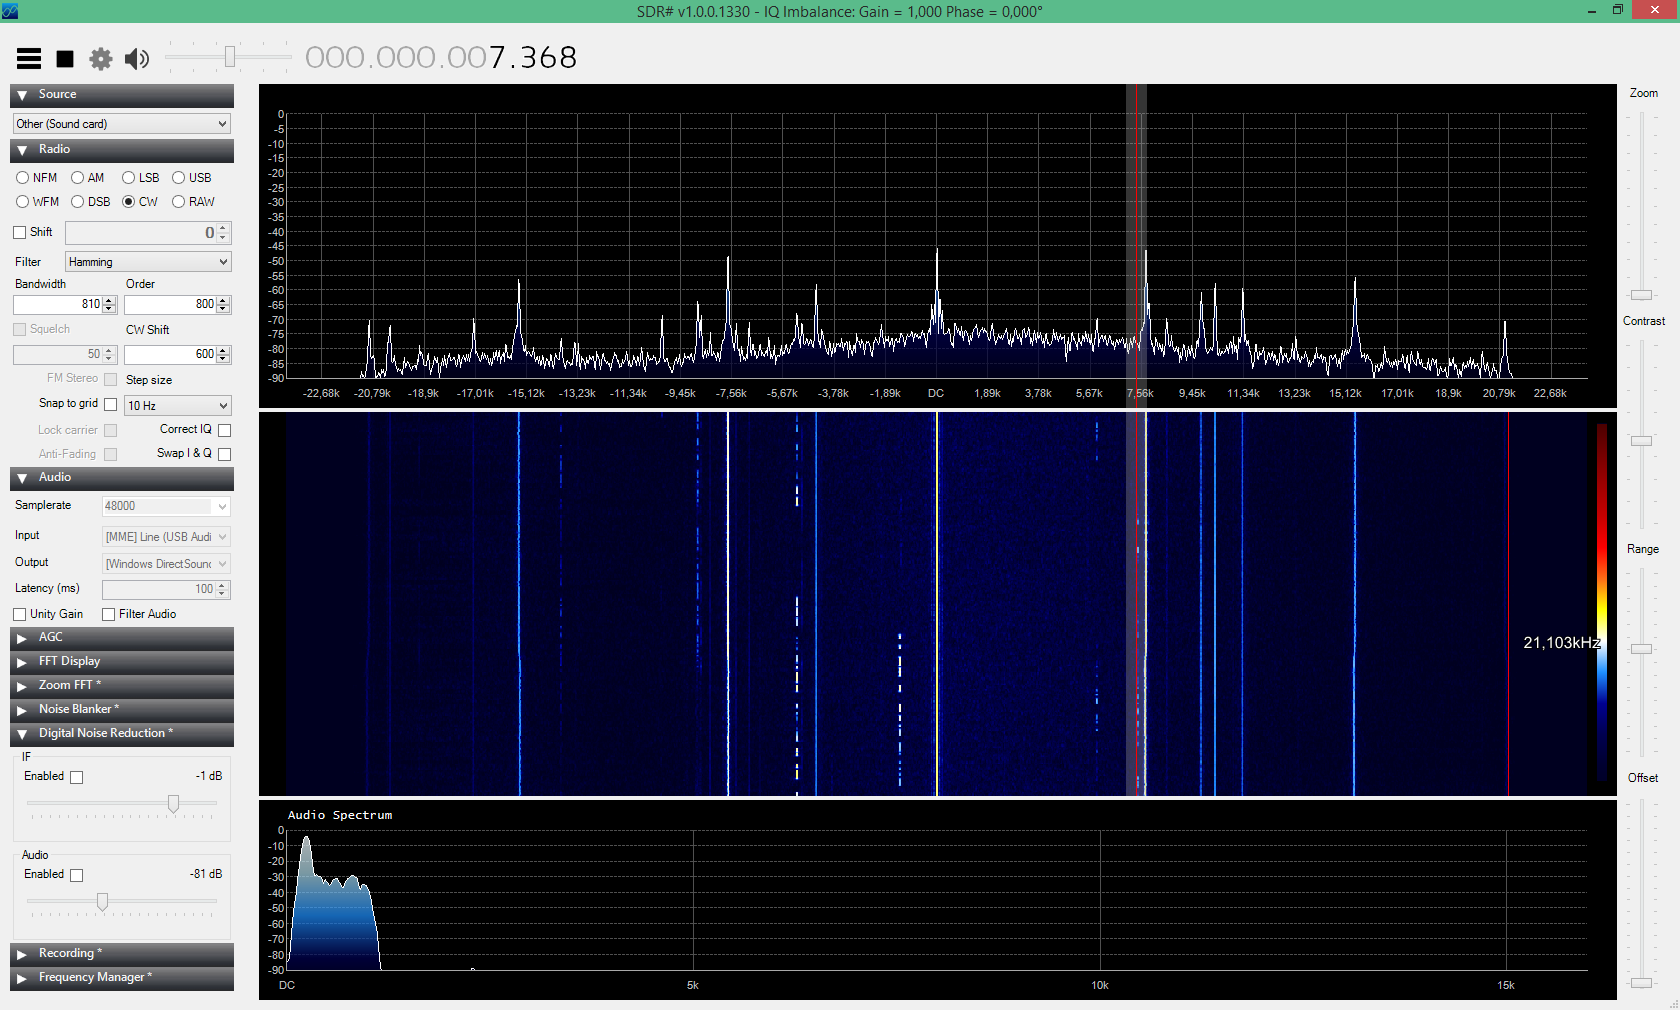
\includegraphics[width=170mm]{img/prijem.png}
	\caption{Ukázka příjmu telegrafie na kmitočtu $14.01~MHz$}    		
\end{figure}

\subsection{Sharp SDR}
\indent\indent Ke zpracovávání signálu jsem si vybral program Sharp SDR. Tento program umožňuje zpracování signálů I a Q ze zvukové karty. Jeho velkou předností je snadné ovládání. Můžeme si zde měnit šířku přijímaného pásma, dokáže demodulavat jak AM modulace, tak také modulace FM. Demodulování CW je samozřejmostí. Dále je možné nastavovat potlačení šumu ve výstupním i vstupním signálu.